\documentclass[11pt]{article}
\newcommand{\Vers}{04 Apr 2023}

\usepackage{graphicx}
\usepackage{amssymb}
\usepackage{amsmath}

\usepackage[html,dvipsnames]{xcolor}


\setlength{\textwidth}{6.5in}
\setlength{\textheight}{9.0in}
\headheight=0.5in
\topmargin=-0.75in
\oddsidemargin= 0.0in
\evensidemargin=-0.25in

\usepackage[
    pdfauthor={Brandon Franzke}, pdftitle={EE 541 Project Proposal}, %
    pdftex, bookmarks
  ]{hyperref} %
    \hypersetup{colorlinks,%
    citecolor=green,%
    filecolor=Orange,%
    linkcolor=blue,%
    urlcolor=BrickRed}

\usepackage{titlesec}
\titleformat*{\section}{\large\bfseries}

\pagestyle{myheadings}
\markright{{\bf EE 541 - \copyright B. Franzke - Spring 2023} }


\title{\bf {\small EE 541 -- Computational Introduction to Deep Learning} \\ Project Proposal}
\author{Eric Liu, Zhenxuan Su}
\date{November 15, 2023}
\begin{document}
\maketitle

\paragraph{Project Title:}  Musical Chord Classification

\section*{Topic summary}


\noindent
We propose to create a model to perform binary classification of musical chords to determine whether a chord is major or minor for piano and guitar. 
We will train the model using a dataset of labeled audio samples of piano and guitar chords.
The model will be based on a convolutional neural network (CNN) architecture, which has been shown to be effective in audio classification tasks. 
The CNN will take as input the spectrogram of the audio signal and output a binary classification of the chord as major or minor.   (Figure \ref{fig:waveform}).
We will evaluate the performance of the model using standard metrics such as accuracy, F1 score. 
A successful model will have a high accuracy in classifying musical chords (for piano and guitar) as major or minor, which can be used in multiple applications such as  musical recognition, music recommendation on music applications, and live sheet music generation.

\begin{figure}[!htb]
  \begin{center}
  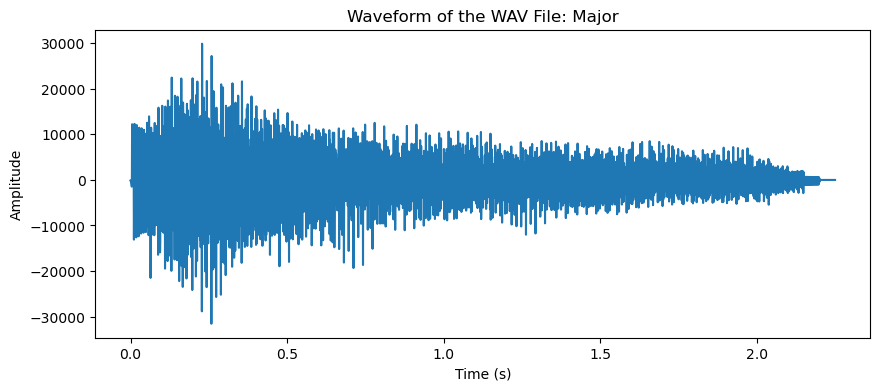
\includegraphics[width=0.75\linewidth]{./Figure/Majorwave.png}
   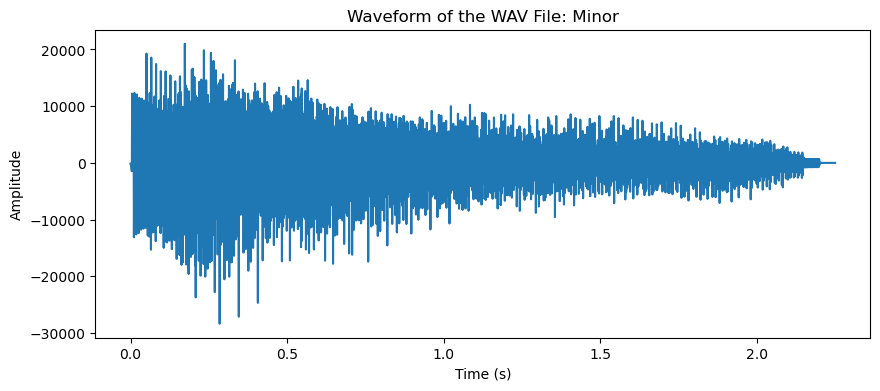
\includegraphics[width=0.75\linewidth]{./Figure/Minorwave.png}
  \caption{Waveform of musical chord.}
  \label{fig:waveform}
  \end{center}
  \vspace{-0.6cm}
\end{figure}

\section*{Introduction}

\begin{itemize}
\item The ability to accurately classify chords as major or minor can have a significant impact on the field of music and can benefit a wide range of people. It will help musicians to automatically do transcription of sheet music, which reduce the workload. Also, it will help music teachers and students to tag the mistake of playing instruments, and do auto-grade for the assignments. In the music industry, digital music providers like Spotify, Apple Music, etc., can benefit from using chord classification to recommend new songs for users based on their preferences or to recognize songs for users.
\item \textbf{Note}: the most fundamental building block of music. There are 7 natural notes, represented as do-re-mi-fa-sol-la-si or A-B-C-D-E-F-G, which can be played with white keys on a piano. In between these natural notes are 5 half-step notes (e.g. A\# between $A$ and B) except B-C and E-F. They can be played with black keys on a piano. In total, there are 12 notes listed as follows and each pair of adjacent notes are half-step apart.

A A\# B C C\# D D\# EFF\# G G\#
\item \textbf{Frequency}: each note has a corresponding frequency $(\mathrm{Hz})$ that can be calculated as
$$
f=440 \cdot 2^{d / 12}
$$
where $d$ is the number of half-steps away from the reference note $\mathrm{A}$.

        \item  \textbf{Chord}: a harmonic set of notes/frequencies that are heard as if sounding simultaneously. A major chord consists of a root note, a major third (4 half-steps higher than the root), and a perfect fifth (7 half-steps higher than the root). A minor chord consists of a root note, a minor third (3 half-steps higher than the root), and a perfect fifth. For example, if the root is $\mathrm{C}$, then the major chord is $\mathrm{C}-\mathrm{E}-\mathrm{G}$ and the minor chord is $C-D \#-G$.
  

\end{itemize}

\section*{Related Work}

\begin{itemize}
  \item Who else has worked on this problem before? There are some project about chord classification, Ahmet Celik used a feature extraction method called voiced models to recognize chords in the music, which performed better than manual feature extraction. They also used traditional classification to create the key classifier, which was better than other classifiers. 
  \item What did they find? The project’s author, Ahmet Celik, uses the discrete and continuous Fourier transforms to extract important information from audio data. The overall accuracy is about 94%.
  \item How does the related work compare to your proposed topic? We both need to implement Fourier transforms to extract important information, however, we are trying to use CNN to solve the problem more efficiently.
\end{itemize}

\section*{Dataset description}

\href
{https://www.kaggle.com/datasets/deepcontractor/musical-instrument-chord-classification}
{https://www.kaggle.com/datasets/deepcontractor/musical-instrument-chord-classification}

\vspace{0.3cm}

\noindent
The dataset is 142 MB.
It consists of 502 major chord files and 357 minor chord files.
Each file is a single-channel wav file of 2-3 seconds with sample rate 44100Hz. We split the data into train/validation/test sets.

As the raw data is in time domain, we will preprocess it into frequency domain and experiment on models taking time domain data and frequency domain data as input, respectively and compare their performance.

\section*{Objective}
The objective of this project is perform a binary classification to determine whether a chord is major or minor for piano and guitar.

We will measure model performance using two metrics, which are the accuracy and log-likelihood given by
\begin{displaymath}
  L = \frac{1}{N}\sum\limits_{i=1}^{N}y_i\log(\hat{y}_i) + (1 - y_i) \log(1 - \hat{y}_i),
\end{displaymath}
where $y_i$ is the true label of the i-th data and $\hat{y}_i$ is the prediction of model.


\section*{Investigation Plan}
Distinguishing ideal chords is easy because they are composition of impulse in frequency domain. We will first visualize some of the data, try to perform a non-ML classification algorithm as baseline and conclude how ML can improve. 


\section*{Estimated Compute Needs}

Summarize the compute resources that you intend to use.
We will not use a massive dataset, so PC is enough. Our team will use a Windows PC (with AMD R7, NVIDIA 2060, 16G RAM) and a Mac (with M2 chip,  8G RAM) to train the model.


\section*{Likely Outcome and Expected Results}
We expect to perform the binary classification with accuracy higher than the non-ML baseline on our dataset. And we want to observer difference in performance on time-domain model and frequency-domain model and conclude reasonable interpretations.

The most possible reason for the failure is that we did not design the architecture properly and wasted all the time training it with no good outcomes.


\section*{Primary References and Codebase}

We propose to build on the approach used in

\begin{itemize}
  \item
  Ahmet Çelik, "\href{https://www.kaggle.com/code/ahmetcelik158/mathematics-of-music-chord-classification}{Mathematics of Music: Chord Classification}," Kaggle.

  \item
  Heng-Tze C., Yi-Hsuan Y., Yu-Ching Lin, I-Bin L. and H. H. Chen,  {Automatic chord recognition for music classification and retrieval}. 2008 IEEE International Conference on Multimedia and Expo, Hannover, Germany, 2008, pp. 1505-1508, doi: 10.1109/ICME.2008.4607732.

\end{itemize}

 \end{document}
